\documentclass[tikz,border=10pt]{standalone}
\usepackage{tikz}
\usetikzlibrary{angles,quotes,calc, intersections}

\begin{document}
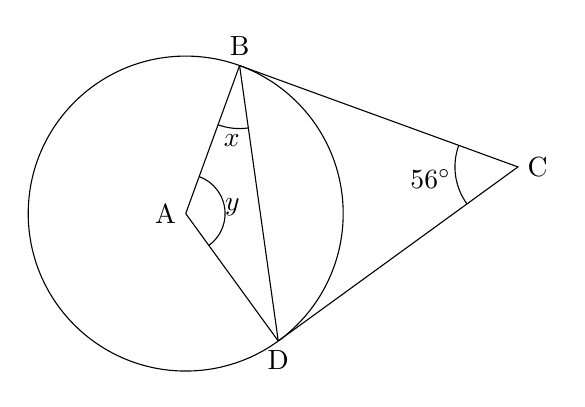
\begin{tikzpicture}

    % Define the center of the circle
    \coordinate (A) at (0,0);
    
    % Draw the circle
    \draw[name path=circ] (A) circle (2cm);

    % Place points B on the circumference
    \coordinate (B) at ($(A) + (70:2cm)$);
    
    \draw (A) -- (B);
    \path[name path = BD] (B) -- ($(B)!2!28:(A)$);
    
   
    % Find intersection point C
    \path [name intersections={of=BD and circ,by={D}}];
    \draw (B) -- (D);
    \draw (A) -- (D);

     % Draw points A,B, and D
    \node at (A) [anchor = east] {A};
    \node at (B) [anchor = south] {B};
    \node at (D) [anchor = north] {D};
    
    % % Draw tangent lines
    \path[name path = BC] (B) -- ($(B)!2!90:(A)$);
    \path[name path = DC] (D) -- ($(D)!2!-90:(A)$);
    \path [name intersections={of=BC and DC,by={C}}];
    \draw (B) -- (C) -- (D);
    % Label point C
    \node at (C) [right] {C};
    
    \pic [draw, "$x$", angle eccentricity=1.2, angle radius = 0.8cm] {angle = A--B--D};
    \pic [draw, "$y$", angle eccentricity=1.2, angle radius = 0.5cm] {angle = D--A--B};
    \pic [draw, "$56^\circ$", angle eccentricity=1.4, angle radius = 0.8cm] {angle = B--C--D};

\end{tikzpicture}
\end{document}
